\documentclass{beamer}
\usepackage{beamerthemesplit}
\usetheme{SPbGU}
%{CambridgeUS}
% Выпишем часть возможных стилей, некоторые из них могут содержать
% дополнительные опции
% Darmstadt, Ilmenau, CambridgeUS, default, Bergen, Madrid, AnnArbor,Pittsburg, Rochester,
% Antiles, Montpellier, Berkley, Berlin
\usepackage{pdfpages}
\usepackage{amsmath}
\usepackage{cmap} % for serchable pdf's
\usepackage[T2A]{fontenc} 
\usepackage[utf8]{inputenc}
\usepackage[english,russian]{babel}
\usepackage{indentfirst}
\usepackage{amsmath}
\usepackage{dot2texi}
\usepackage{tikz}
\usepackage{graphicx}
\usetikzlibrary{shapes,arrows}
\usepackage{fancyvrb}
\usepackage{graphicx}
\usepackage{array}
\usepackage{color}


% Если у вас есть логотип вашей кафедры, факультета или университета, то
% его мож но включить в презентацию.

%\usefoottemplate{\vbox{}}%  \tinycolouredline{structure!25}% {\color{white}\textbf{\insertshortauthor\hfill% \insertshortinstitute}}% \tinycolouredline{structure}% {\color{white}\textbf{\insertshorttitle}\hfill}% }}

%\logo{
\includegraphics[width=1cm]{SPbGU_Logo.png}}

%[GLR-анализатор]
\title[]{From abstract parsing to abstract translation}
\subtitle[]{Research project}
\institute[SPbSU]{
Saint-Petersburg State University \\
The faculty of Mathematics and Mechanics }



\author[Semyon Grigorev]{Grigorev Semyon}

\date{29.05.2014}

\begin{document}
{

\begin{frame}
\begin{center}
{
\includegraphics[width=1cm]{SPbGU_Logo.png}}
\end{center}
%\frame{ 
\titlepage
%}
\end{frame}
}

\definecolor{orange}{RGB}{179,36,31}


\begin{frame}[fragile]
	\transwipe[direction=90]
	\frametitle{String-embedded languages}
	\begin{itemize}
		\item Dynamic SQL
		\begin{Verbatim}[commandchars=\\\{\}]
\textcolor{blue}{IF} @X = @Y
    \textcolor{blue}{SET} @TABLE = \textcolor{orange}{'#table1'}
\textcolor{blue}{ELSE}
    \textcolor{blue}{SET} @TABLE = \textcolor{orange}{'table2'}
\textcolor{blue}{EXECUTE} 
    (\textcolor{orange}{'SELECT x FROM'} + @TABLE + \textcolor{orange}{' WHERE ISNULL(n,0) > 1'})
		\end{Verbatim}
		\item JavaScript in Java
		\begin{Verbatim}[commandchars=\\\{\}]
\textcolor{blue}{String} script =
    \textcolor{orange}{"function hello(name) { print(’Hello, ’ + name); }"};
engine.eval(script);
\textcolor{blue}{Invocable} inv = (\textcolor{blue}{Invocable}) engine;
inv.invokeFunction(\textcolor{orange}{"hello"}, \textcolor{orange}{"Scripting!!!"} );
        \end{Verbatim}
	\end{itemize}
\end{frame}


\begin{frame}
	\transwipe[direction=90]
	\frametitle{Problems}	
	\begin{itemize}
		\item Strings are expressions in programming language
		\begin{itemize}
		    \item They can contain errors
		    \item It may be necessary to transform them
   		    \item Any other problems of programming languages may occure
    	\end{itemize}
	\end{itemize}
\end{frame}

\begin{frame}
	\transwipe[direction=90]
	\frametitle{Related work}
	\begin{itemize}
		\item Kyung-Goo Doh, Hyunha Kim, David A. Schmidt
			\begin{itemize}
			    \item Combination of LR-based parsing algorithm and data-flow analysis to process string-embedded languages
    			\begin{itemize}
			        \item We try to parse an approximation of set of dymaically constructed expression: data-flow equation, \textbf{graph}, etc
            	\end{itemize}
			    \item We can use attributed grammars to specify semantics actions
			    \item Naive implementation of proposed algorithm has performance and space issues
        	\end{itemize}
    	\item Alvor, Java String Analyzer, PHP String Analyzer are not usable for transformations
	\end{itemize}
\end{frame}

\begin{frame}[fragile]
	\transwipe[direction=90]
	\frametitle{Approximation}
	\begin{itemize}
	\item
		\begin{Verbatim}[commandchars=\\\{\}]
\textcolor{blue}{IF} @X = @Y
    \textcolor{blue}{SET} @TABLE = \textcolor{orange}{'#table1'}
\textcolor{blue}{ELSE}
    \textcolor{blue}{SET} @TABLE = \textcolor{orange}{'table2'}
\textcolor{blue}{EXECUTE} 
    (\textcolor{orange}{'SELECT x FROM '} + @TABLE + \textcolor{orange}{' WHERE ISNULL(n,0) > 1'})
		\end{Verbatim}
     	\item Set of values: \\ \{'SELECT x FROM \#table1 WHERE ISNULL(n,0) > 1' ; \\ \vspace{2pt} 'SELECT x FROM table2 WHERE ISNULL(n,0) > 1'\}
    	\item Approximation: 
            %\begin{center}
                \includegraphics[width = 0.9\textwidth]{./dot/approximation1.eps}
            %\end{center}

	\end{itemize}
\end{frame}

\begin{frame}
	\transwipe[direction=90]
	\frametitle{Real world example}
    DBMS migration from MS-SQL (T-SQL) to Oracle server (PL-SQL)
    \begin{itemize}
       \item > 2 mln lines of code
       \item ~3000 hotspots (EXECUTE(string) statements)
       \begin{itemize}
           \item More than 50\% of them can have more than one value
           \item 212 is a maximum number of expression-generating operators for one expression
           \item 40 is average number of expression-generating operators
       \end{itemize}
       \pause
       \item > 16 Gb RAM in use and not finished in 5 hours because we get a huge number of trees
    \end{itemize}
\end{frame}

\begin{frame}
	\transwipe[direction=90]
	\frametitle{Solution}
  Run time parsing results filtration
  \begin{itemize}
   \item Stacks filtration
   \item Forest filtration
  \end{itemize}
\end{frame}

\begin{frame}
	\transwipe[direction=90]
	\frametitle{Forest minimization}
    \begin{figure}
    \centering
    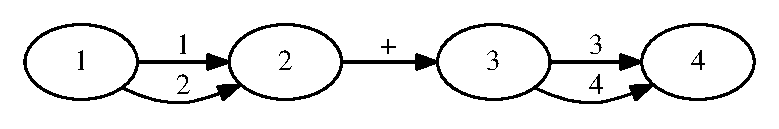
\includegraphics[width = 0.9\textwidth]{./dot/input1.eps}
  \end{figure}
  \begin{center}
  \begin{tabular}{c | c}
      \includegraphics[width = 0.4\textwidth]{./dot/tree1.eps}      
      &
      \includegraphics[width = 0.4\textwidth]{./dot/tree2.eps}
      \\
      \hline
      \includegraphics[width = 0.4\textwidth]{./dot/tree3.eps}      
      &
      \includegraphics[width = 0.4\textwidth]{./dot/tree4.eps}

  \end{tabular}
    \end{center}
\end{frame}

\begin{frame}
	\transwipe[direction=90]
	\frametitle{Forest minimization}
    \begin{figure}
    \centering
    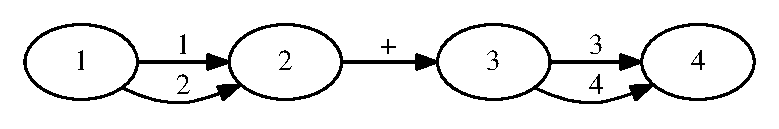
\includegraphics[width = 0.9\textwidth]{./dot/input1.eps}
  \end{figure}
  \begin{center}
  \begin{tabular}{c  c}
      \fcolorbox{red}{white}{\includegraphics[width = 0.4\textwidth]{./dot/tree1.eps}}
      &
      \fcolorbox{green}{white}{\includegraphics[width = 0.4\textwidth]{./dot/tree2.eps}}
      \\
     
      \fcolorbox{green}{white}{\includegraphics[width = 0.4\textwidth]{./dot/tree3.eps}}
      &
      \fcolorbox{red}{white}{\includegraphics[width = 0.4\textwidth]{./dot/tree4.eps}}

  \end{tabular}
    \end{center}
\end{frame}

\begin{frame}
	\transwipe[direction=90]
	\frametitle{Forest filtration}
	\begin{itemize}
	\item Runtime filtration in each vertice with multiple input edges
	\begin{itemize}
    	\item Results with unique parser states
    	\item Minimal set of paths which contains all edges
	\end{itemize}
    \item Why not static filtration of input graph?
    \item We can not predict path correctness 
	\end{itemize}
\end{frame}

\begin{frame}
	\transwipe[direction=90]
	\frametitle{Static selection problem}
	\begin{itemize}
	\item Possible result of static paths selection: \\ {\includegraphics[width = 0.4\textwidth]{./dot/static1.eps}}
	\begin{itemize}
    	\item All selected paths are incorrect
    	\item No trees in result
	\end{itemize}
	\pause
	\item Seems we should select other set of paths.\\
	{\includegraphics[width = 0.4\textwidth]{./dot/static2.eps}}
	\begin{itemize}
    	\item 2 correct trees
    	\item All variables are used
	\end{itemize}
	\end{itemize}
\end{frame}


\begin{frame}
	\transwipe[direction=90]
	\frametitle{Conclusion}
	Described algorithm was implemented and used for migration of production system
	\begin{itemize}
	    \item Full processing in 2 hours
		\item Fully processed expressions: 2181 $\rightarrow$ 2253
		\item Finished by timeout (not processed): 253 $\rightarrow$ 42
       % \item Not automatic processing. Automatization only
        \item It is possible to use ideas of GLR to improve our algorithm
	\end{itemize}
\end{frame}

\begin{frame}
	\transwipe[direction=90]
	\frametitle{Contact Information}
	\begin{itemize}
        \item Grigorev Semyon: Semen.Grigorev@jetbrains.com
		\item YaccConstructor: \href{http://recursive-ascent.googlecode.com}{http://recursive-ascent.googlecode.com}
	\end{itemize}
\end{frame}

\end{document}
